%GiG
\documentclass{beamer} 
\usetheme{Copenhagen}
\setbeamertemplate{navigation symbols}{}
\setbeamertemplate{headline}{}
\DeclareMathOperator*{\argmax}{arg\,max}

\usepackage{hyperref}
\definecolor{azure}{rgb}{0.0, 0.5, 1.0}
%\newcommand{\tblue}[1]{\textcolor{blue}{#1}}
\newcommand{\tblue}[1]{{\Large {\textcolor{azure}{#1}}}}
\newcommand{\hred}[1]{{\textcolor{red}{#1}}}

\title[Saravanan Thirumuruganathan] 
{Lecture 5: Binary Search, Introduction to Data Structures for Dynamic Sets}

\author[CSE 5311] 
{Instructor: Saravanan Thirumuruganathan}

\date[] 

\begin{document}

\begin{frame}
  \titlepage
\end{frame}

%\begin{frame}{Outline}
%  \tableofcontents
%  % You might wish to add the option [pausesections]
%\end{frame}

\section{Outline}

\begin{frame}
\frametitle {Outline}
\begin{enumerate}
\item Search problem - Linear and Binary Search
\item Data Structures for representing Dynamic Sets
\begin{itemize}
    \item Linear
    \item Non-Linear/Hierarchical 
\end{itemize}
\end{enumerate}
\end{frame}

\begin{frame}{In-Class Quizzes}
\begin{itemize}
\item {\Large {\bf URL:}} {\LARGE \bf \url{http://m.socrative.com/}} 
\item {\Large {\bf Room Name:} {\LARGE \bf 4f2bb99e}}
\end{itemize}
\end{frame}

\section{Search Problem}


\begin{frame}{Search Problem}

\tblue{Search Problem}
\begin{itemize}
\item {\bf Input:} Set $A$ with $n$ numbers and an element $e$
\item {\bf Output:} First index of $e$ in $A$
\item {\bf Example:} $A = \langle 3, 2, 4, 1, 6, 8, 11 \rangle$, $e=4$. Output=$3$
\end{itemize}
\end{frame}


\begin{frame}{Linear Search}
\begin{itemize}
\item Also called as Sequential search
\item Idea: Examine each element in $A$ one by one from start to finish
\item Always works - whether $A$ is sorted or not
\item Analysis: \pause
\begin{itemize}
    \item Complexity Measure: Number of comparisons
    \item Time Complexity: $O(n)$
\end{itemize}
\end{itemize}
\end{frame}



\begin{frame}{Searching in a Sorted Set}
\begin{itemize}
\item If the application is search intensive, then sorting is a good idea
\item If you do linear Search of $A$ for $n$ times then it requires $O(n^2)$ time
\item We can do better!
\end{itemize}
\end{frame}



\begin{frame}{Binary Search Intuition}
\begin{itemize}
\item Intuition 1: Searching for a word in a dictionary \pause
\begin{itemize}
    \item Check the middle of the book
    \item Proceed in one direction based on the middle page
    \item Recurse
\end{itemize}
\item Intuition 2: Guessing game \pause
\begin{itemize}
    \item Your friend wants thinks of a number between $1$ and $n$ 
    \item You have to find it in least number of guesses
    \item When you make a guess, your friend tells {\em Yes}, {\em Lower} or {\em Higher}
    \item Use the information to cut the search space
\end{itemize}
\end{itemize}
\end{frame}



\begin{frame}{Binary Search}
\begin{itemize}
\item {\em Very} popular searching technique
\item Based on D\&C technique
\item At each step, cut your search space by half
\item {\bf High Level Idea:}
\begin{itemize}
    \item Get midpoint of range (aka search space)
    \item Determine which half contains the data
    \item Search that half recursively using Binary search
\end{itemize}
\end{itemize}
\end{frame}



\begin{frame}[fragile]{Binary Search}
\begin{verbatim}
BinarySearch(A, e, low, high):
    if low > high
        return Not found
    else
        mid = (low + high) / 2
        if e == A[mid]
            return mid
        else if e < A[mid]
            return BinarySearch(A, e, low, mid - 1)
        else 
            return BinarySearch(A, e, mid+1, high)
\end{verbatim}
\end{frame}


\begin{frame}{Binary Search Analysis}
\begin{itemize}
\item {\bf Analysis:} Given a set with $n$ elements - at each iteration, 
\begin{itemize}
    \item You do one comparison
    \item Recursively call  Binary Search with $n/2$ elements 
\end{itemize}
\item $n \rightarrow \frac{n}{2} \rightarrow \frac{n}{4} \rightarrow \ldots \rightarrow 8 \rightarrow 4 \rightarrow 2 \rightarrow 1$
\pause
\item Requires at the most $\lceil \lg n \rceil$ comparisons
\item Time Complexity: $O(\lg n)$
\end{itemize}
\end{frame}

\begin{frame}{Practical Issues}
\begin{itemize}
\item Despite simplicity, very hard to get the implementation right! 
\item Bentley
\begin{itemize}
    \item Bell Labs story - only 10\% of engineers got it right after 2 hours! 
    \item Java story - If interested, read \url{http://googleresearch.blogspot.com/2006/06/extra-extra-read-all-about-it-nearly.html}
    \item Issues found in C, C++, Java etc
    \item If interested, read (from UTA network) \url{http://comjnl.oxfordjournals.org/content/26/2/154.full.pdf} 
\end{itemize}
\item Moral of the story: Don't implement it yourself - Always use from language library!
\end{itemize}
\end{frame}


\section{Representing Dynamic Sets}

\begin{frame}{Data Structures}
\begin{center}
    {\Huge {\textcolor{azure}{Data Structures}}}
\end{center}
\end{frame}


\begin{frame}{Data Structures}

\tblue{Key Points:}
\begin{itemize}
\item What is the objective? 
\begin{itemize}
    \item Store the input data
    \item Help make an algorithm faster (by storing intermediate data)
    \item Transform input to make queries faster
\end{itemize}
\item Is there a specific property/constraint to satisfy?
\item List of operations to support
\item List of most important operations
\end{itemize}
\end{frame}


\begin{frame}{Dynamic Sets}
\begin{itemize}
\item {\bf Set:}  A set is a collection of distinct objects
\item {\bf Dynamic Set:} A set that changes over time (grow or shrink)
\item {\bf Objective:} Design an efficient data structure to represent a dynamic set
\end{itemize}
\end{frame}


\begin{frame}{Operations on Dynamic Sets}
\begin{itemize}
\item Search($S, k$) 
\item Insert($S, x$)
\item Delete($S, x$)
\item Minimum($S$)
\item Maximum($S$)
\item Successor($S, x$)
\item Predecessor($S, x$)
\end{itemize}
\end{frame}


\begin{frame}{Dictionary}

\tblue{Dictionary:}
\begin{itemize}
\item Insert
\item Delete
\item Test membership (Search)
\end{itemize}
\end{frame}


\begin{frame}{Elements of Dynamic Set}
\begin{itemize}
\item {\bf Key:} A set of attributes that identify an object 
\begin{itemize}
    \item Only Key is used by set maintenance algorithms
\end{itemize}
\item {\bf Satellite Information:} Auxiliary information about the object not used by the algorithms
\begin{itemize}
    \item Not used by set maintenance algorithms
\end{itemize}
\end{itemize}
\end{frame}


\begin{frame}{Elementary Data Structures}

\tblue{Linear Data Structures:}
\begin{itemize}
\item Unordered List 
\item Ordered List 
\item (Doubly) Linked Lists
\item (Doubly) Sorted Linked Lists
\end{itemize}
\end{frame}


\begin{frame}{Unordered List}
\begin{center}
    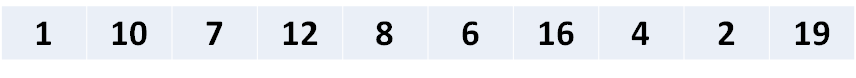
\includegraphics[scale=0.4]{list.png}
\end{center}
\begin{itemize}
    \item Search
    \item Insert
    \item Delete
    \item Minimum/Maximum
    \item Successor/Predecessor
\end{itemize}
\end{frame}


\begin{frame}{Unordered List}
\begin{center}
    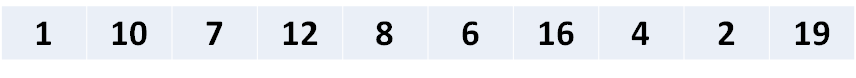
\includegraphics[scale=0.4]{list.png}
\end{center}
\begin{itemize}
    \item Search : $O(n)$
    \item Insert : $O(1)$ 
    \item Delete: $O(n)$
    \item Minimum/Maximum $O(n)$
    \item Successor/Predecessor: $O(n)$
\end{itemize}
\end{frame}



\begin{frame}{Ordered List}
\begin{center}
    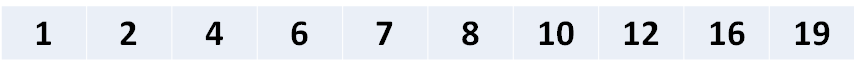
\includegraphics[scale=0.4]{orderedList.png}
\end{center}
\begin{itemize}
    \item Search
    \item Insert
    \item Delete
    \item Minimum/Maximum
    \item Successor/Predecessor
\end{itemize}
\end{frame}


\begin{frame}{Ordered List}
\begin{center}
    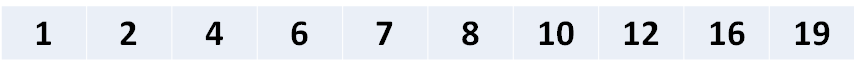
\includegraphics[scale=0.4]{orderedList.png}
\end{center}
\begin{itemize}
    \item Search : $O(\lg n)$
    \item Insert: $O(n)$
    \item Delete: $O(n)$
    \item Minimum/Maximum $O(1)$
    \item Successor/Predecessor: $O(\lg n)$
\end{itemize}
\end{frame}



\begin{frame}{Unordered Doubly Linked List}
\begin{center}
    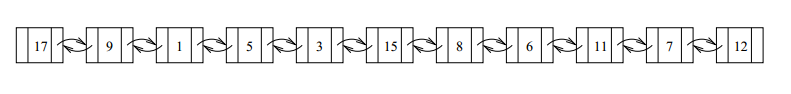
\includegraphics[scale=0.4]{linkedList.png}
\end{center}
\begin{itemize}
    \item Search
    \item Insert
    \item Delete
    \item Minimum/Maximum
    \item Successor/Predecessor
\end{itemize}
\end{frame}


\begin{frame}{Unordered Doubly Linked List}
\begin{center}
    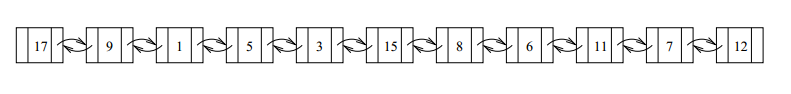
\includegraphics[scale=0.4]{linkedList.png}
\end{center}
\begin{itemize}
    \item Search : $O(n)$
    \item Insert: $O(1)$
    \item Delete: $O(n)$
    \item Minimum/Maximum $O(n)$
    \item Successor/Predecessor: $O(n)$
\end{itemize}
\end{frame}



\begin{frame}{Ordered Doubly Linked List}
\begin{center}
    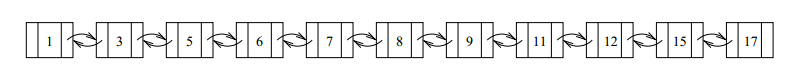
\includegraphics[scale=0.4]{orderedLinkedList.png}
\end{center}
\begin{itemize}
    \item Search
    \item Insert
    \item Delete
    \item Minimum/Maximum
    \item Successor/Predecessor
\end{itemize}
\end{frame}


\begin{frame}{Ordered Doubly Linked List}
\begin{center}
    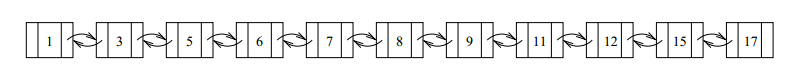
\includegraphics[scale=0.4]{orderedLinkedList.png}
\end{center}
\begin{itemize}
    \item Search : $O(n)$
    \item Insert: $O(n)$
    \item Delete: $O(n)$
    \item Minimum/Maximum $O(n)$
    \item Successor/Predecessor: $O(n)$
\end{itemize}
\end{frame}



\section{Summary}
\begin{frame}{Summary}

\tblue{Major Concepts:}
\begin{itemize}
\item Search Problem
\item Linear and Binary Search algorithms
\item Data Structures for Dynamic Sets
\end{itemize}
\end{frame}


\end{document}

